\documentclass[conference]{IEEEtran}
\IEEEoverridecommandlockouts
% The preceding line is only needed to identify funding in the first footnote. If that is unneeded, please comment it out.
\usepackage{cite}
\usepackage{amsmath,amssymb,amsfonts}
\usepackage{algorithmic}
\usepackage{graphicx}
\usepackage{textcomp}
\usepackage{xcolor}
\usepackage{subfig}
\usepackage{multirow}
\usepackage{booktabs}

\def\BibTeX{{\rm B\kern-.05em{\sc i\kern-.025em b}\kern-.08em
    T\kern-.1667em\lower.7ex\hbox{E}\kern-.125emX}}
    
\usepackage[nomain, toc, acronym]{glossaries}
\glsdisablehyper

\newcommand\note[2]{{\color{#1}#2}}
\newcommand\todo[1]{{\note{red}{TODO: #1}}}

\newcommand{\unsw}{UNSW-NB15}
\newcommand{\cic}{CIC-IDS-2017}

\newacronym{dl}{DL}{Deep Learning}
\newacronym{ad}{AD}{Anomaly Detection}
\newacronym{ml}{ML}{Machine Learning}
\newacronym{ttl}{TTL}{Time-to-Live}
\newacronym{ids}{IDS}{Intrusion Detection System}
\newacronym{mlp}{MLP}{Multilayer Perceptron}
\newacronym{relu}{ReLU}{Rectified Linear Unit}
\newacronym{ip}{IP}{Internet Protocol}
\newacronym{ffnn}{FNN}{Feedforward Neural Network}

\begin{document}

%\title{EagerNet: Early Intrusion Prediction\\in Feed Forward Neural Networks}
\title{EagerNet: Early Predictions in Feedforward Neural Networks for Fast Network Intrusion Detection}

\author{\IEEEauthorblockN{Fares Meghdouri, Maximilian Bachl and Tanja Zseby}
\IEEEauthorblockA{Technische Universität Wien\\
Vienna, Austria\\
firstname.lastname@tuwien.ac.at}}



\maketitle

\begin{abstract}

\glspl{ffnn} have been the basis of most state-of-the-art \gls{ml} applications in recent years. Experiments show that the deeper the network is, the more desirable it is to acquire more knowledge. Nonetheless, with the growing number of layers, obtaining fast predictions has become a difficult task despite the use of special hardware such as GPUs. We propose a new architecture to obtain predictions without conducting a forward-pass until the last layer. The architecture is able to deal with either binary or multiclass classification problems and trades prediction speed for the confidence of the network. We evaluate our proposal with two different network intrusion detection datasets. Results suggest that it is possible to obtain comparable accuracies to simple \glspl{ffnn} without evaluating all layers, thus obtaining early predictions and saving energy and computational efforts.

\end{abstract}

\begin{IEEEkeywords}

\end{IEEEkeywords}

\section{Introduction}
% what are ffnn
\glspl{ffnn} has gained remarkable attention in recent years due to the availability of data and computational resources for research. Many of the state-of-the-art architectures currently used in different applications are effectively based on simple \glspl{ffnn} architectures. Experiments show that the more layers (and neurons) the network includes, the more desirable it is for better learning \cite{eldan2016power} .

% forward-backward
Traditional \gls{ffnn} are based on simple logistic regression units that combine multiple inputs multiplied by a set of weights and passed through an activation function (e.g. sigmoid) to obtain a scalar. The weights are adjusted to give the closest possible output to a ground-truth. As far as neural networks are concerned, logistic regression units are stacked together to create layers and then layers are stacked together again to create the network itself. Figure \ref{fig:ffnn} demonstrates a basic \gls{ffnn} that utilizes the input vector $\lbrace X_{1}, X_{2} ... X_{m} \rbrace$ and makes a prediction. Adjusting weights in such situations is a non-trivial problem since the weights of each layer may have an impact on the previous layers. Fortunately, several algorithms have been proposed to reduce the complexity of the task (e.g. gradient descent learning) while achieving the same goal: reduce the "gap" (loss) between predictions and actual desired output. Larger networks consist of more neurons and thus more weights, allowing more data patterns to be learned.

% problem with large networks
In terms of efficiency, two problems arise when using an extremely deep neural networks: (1) The loss during training needs more time to converge and (2) prediction time is proportional to the number of layers. Even though most modern hardware is able to cope with offline single predictions without significant delay, online massive neural network implementations may suffer from the latter issue if non-specialized hardware is used to produce predictions. 
%EagerNet 
To solve this, we propose a new architecture that, on the one hand, uses the entire network capacity for learning and, on the other hand, stops the forward-pass and makes predictions as soon as confidence reaches a certain threshold. In other words, it makes it possible to avoid evaluating the entire network and to receive predictions from intermediate layers with the same performance of a simple \gls{ffnn}. The proposed approach therefore allows, where possible, the reduction of computing resources and energy usage preserving comparable performance of a full forward-pass.

% conclusion
The rest of the paper is organized as follows: In Section ...
 
\section{Supervised Learning for Network Intrusion Detection}

\begin{table}[ht!]
	
	\centering
	\caption{CAIA network flow features.}
	\label{tab:cres}
	     
	\footnotesize
	\begin{tabular}{|c|c|c|}
		\toprule
		\textbf{Direction}                    & \textbf{Features}        & \textbf{Statistical Operations}        \\
		\midrule
		    
		                                      & flowDurationMilliseconds &                                        \\
		                                      & sourceTransportPort      &                                        \\
		                                      & destinationTransportPort &                                        \\
		                                      & protocolIdentifier       &                                        \\
		                                      & octetTotalCount          &                                        \\
		\midrule
		\multirow{7}{*}{Forward and Backward} & ipTotalLength            & \multirow{2}{*}{Mean, Min, Max, Stdev} \\
		                                      & interPacketTimeSeconds   &                                        \\
		\cmidrule{2-3}
		                                      & packetTotalCount         &                                        \\
		                                      & tcpSynTotalCount         &                                        \\
		                                      & tcpAckTotalCount         &                                        \\
		                                      & tcpFinTotalCount         &                                        \\
		                                      & tcpCwrTotalCount         &                                        \\
		   
		\midrule
		
		
	\end{tabular}
		
\end{table}

\section{EagerNet}

\begin{figure*}[htp]
\center
\subfloat[Conventional \gls{ffnn} architecture.]{%
  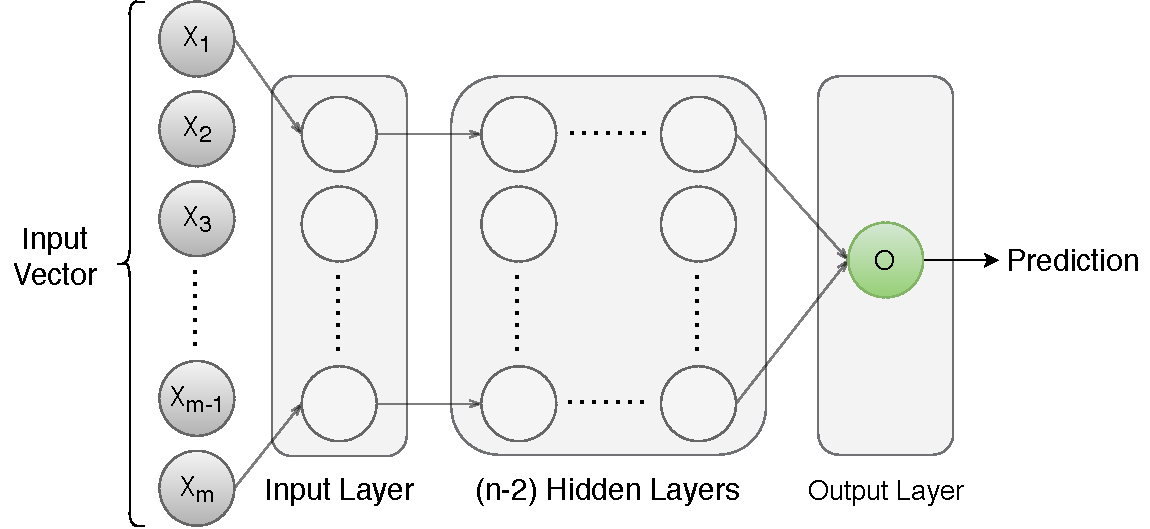
\includegraphics[clip,width=0.45\textwidth]{figures/ffnn_new.pdf}%
  \label{fig:ffnn}
}
\\
\subfloat[EagerNet: Forward-pass.]{%
  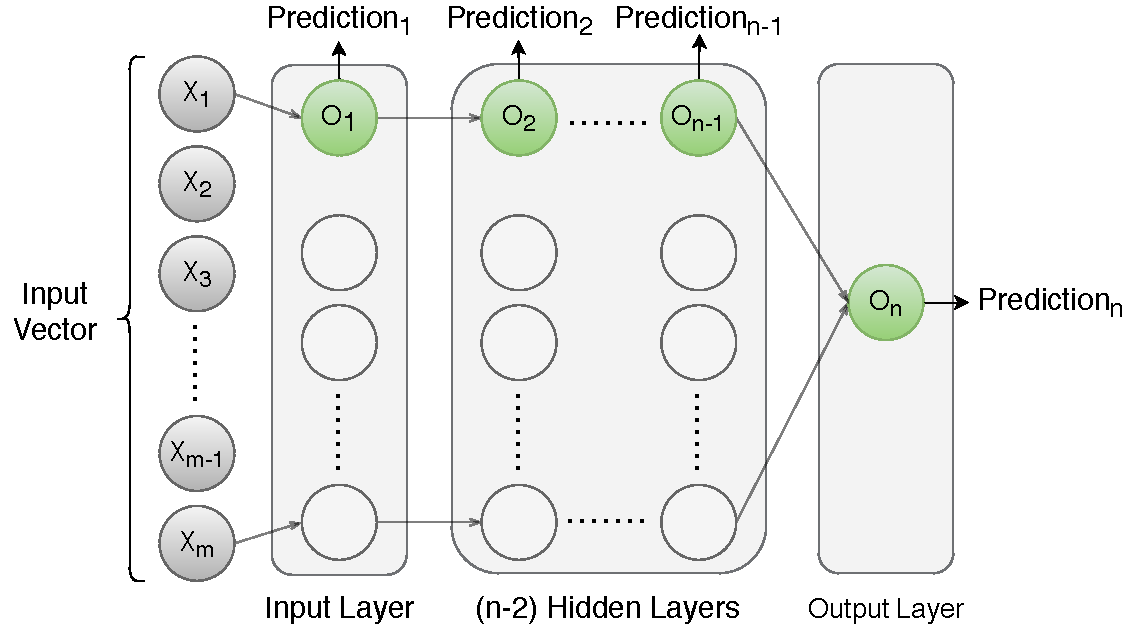
\includegraphics[clip,width=0.53\textwidth]{figures/eagernet_new.pdf}%
}
\quad
\subfloat[EagerNet: Back-propagation of gradients.]{%
  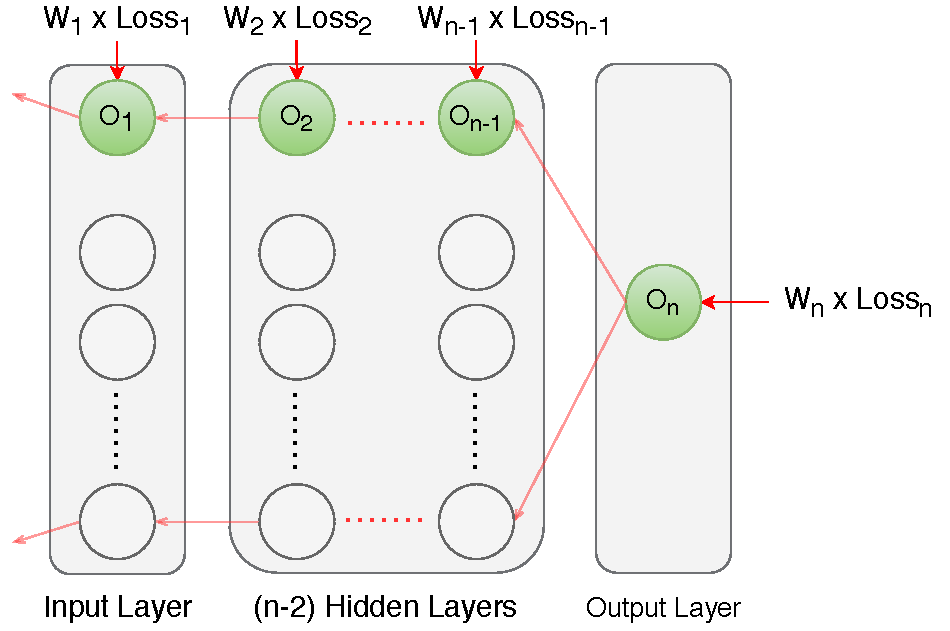
\includegraphics[clip,width=0.45\textwidth]{figures/eagernet_backprop_new.pdf}%
}

\caption{The difference between conventional neural networks and our proposed architecture.}

\end{figure*}

\subsubsection{Binary Vs. Multiclass Classification}

\begin{equation}
l = \frac{1}{N} \sum_{n}^{N} -\omega [y_n \cdot \log \sigma (x_{n}) + (1 - y_n) \cdot \log (1 - \sigma (x_{n}))]
\end{equation}

\[
\nabla l = \underbrace{W_{current} \times \nabla l_{current}}_{\text{Current gradient}} + \underbrace{\sum_{i}^{} \nabla l_{i}}_{\text{Next layer gradients}}
\]

\subsubsection{Combined Back-propagation Loss}

\subsubsection{Design Decision}






\section{Related Work}

\section{Evaluation and Discussion}
\subsection{Datasets}

\subsection{Performance}

\begin{table*}
\parbox{.45\linewidth}{
\centering
\begin{tabular}{cccrrrr}
\toprule
\textbf{Variant} & \textbf{Weights} & \textbf{Layers} & \textbf{Acc.} & \textbf{Prec.} & \textbf{Rec.} & \textbf{J.}\\
\midrule
\multirow{6}{*}{\rotatebox{90}{Binary}} & \multirow{2}{*}{Equal} & 1-3-1 & 0.996 & 0.996 & 0.990 & 0.989 \\
 & & 1-1-1 & 0.997 & 0.997 & 0.990 & 0.990 \\
 & \multirow{2}{*}{Increasing} & 1-3-1 & 0.997 & 0.998 & 0.990 & 0.989 \\
 & & 1-1-1 & 0.997 & 0.997 & 0.990 & 0.989 \\
 & \multirow{2}{*}{Decreasing} & 1-3-1 & 0.997 & 0.998 & 0.989 & 0.989 \\
 & & 1-1-1 & 0.997 & 0.997 & 0.990 & 0.990 \\
\midrule
\multirow{6}{*}{\rotatebox{90}{Multiclass}} & \multirow{2}{*}{Equal} & 1-3-1 & & & & \\
 & & 1-1-1 & & & & \\
 & \multirow{2}{*}{Increasing} & 1-3-1 & & & & \\
 & & 1-1-1 & & & & \\
 & \multirow{2}{*}{Decreasing} & 1-3-1 & & & & \\
 & & 1-1-1 & & & & \\
\end{tabular}
\caption{CIC-IDS17}
}
\hfill
\parbox{.45\linewidth}{
\centering
\begin{tabular}{cccrrrr}
\toprule
\textbf{Variant} & \textbf{Weights} & \textbf{Layers} & \textbf{Acc.} & \textbf{Prec.} & \textbf{Rec.} & \textbf{J.}\\
\midrule
\multirow{6}{*}{\rotatebox{90}{Binary}} & \multirow{2}{*}{Equal} & 1-3-1 & & & & \\
 & & 1-1-1 & & & & \\
 & \multirow{2}{*}{Increasing} & 1-3-1 & & & & \\
 & & 1-1-1 & & & & \\
 & \multirow{2}{*}{Decreasing} & 1-3-1 & & & & \\
 & & 1-1-1 & & & & \\
\midrule
\multirow{6}{*}{\rotatebox{90}{Multiclass}} & \multirow{2}{*}{Equal} & 1-3-1 & & & & \\
 & & 1-1-1 & & & & \\
 & \multirow{2}{*}{Increasing} & 1-3-1 & & & & \\
 & & 1-1-1 & & & & \\
 & \multirow{2}{*}{Decreasing} & 1-3-1 & 0.988 & 0.846 & 0.830 & 0.825 \\
 & & 1-1-1 & & & & \\
\end{tabular}
\caption{UNSW-NB15}
}
\end{table*}



\begin{table}

\centering
\begin{tabular}{ccrr}
\toprule
\textbf{Dataset} & \textbf{Architecture} & \textbf{FFNN} & \textbf{EagerNet*}\\
\midrule
\multirow{6}{*}{\rotatebox{90}{CIC-IDS17}} & & & \\
 & & & \\
 & & & \\
 & & & \\
 & & & \\
 & & & \\
\midrule
\multirow{6}{*}{\rotatebox{90}{UNSW-NB15}} & & & \\
 & & & \\
 & & & \\
 & & & \\
 & & & \\
 & & & \\
\midrule
\multirow{6}{*}{\rotatebox{90}{MNIST}} & & & \\
 & & & \\
 & & & \\
 & & & \\
 & & & \\
 & & & \\
\end{tabular}
\vspace{1ex}

{\raggedright * . \par}
\caption{Accuracy scores.}


\end{table}

\subsection{Confidence-Speed Tradeoff}

\begin{figure}[b!]
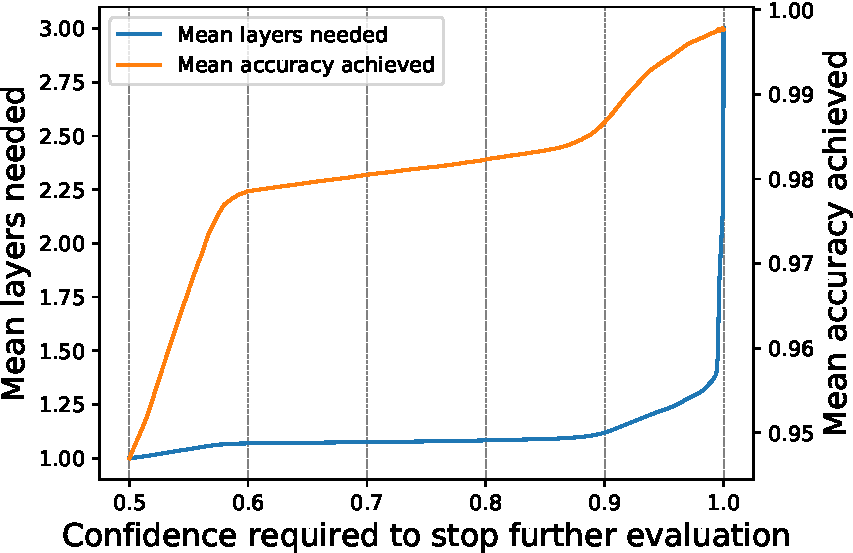
\includegraphics[width=\columnwidth]{figures/conf-acc-layers.pdf}
\caption{Accuracy-Confidence plot.\note{red}{FM: this will change}}
\label{fig:pdp_ttl}
\end{figure}

\begin{figure}[b!]
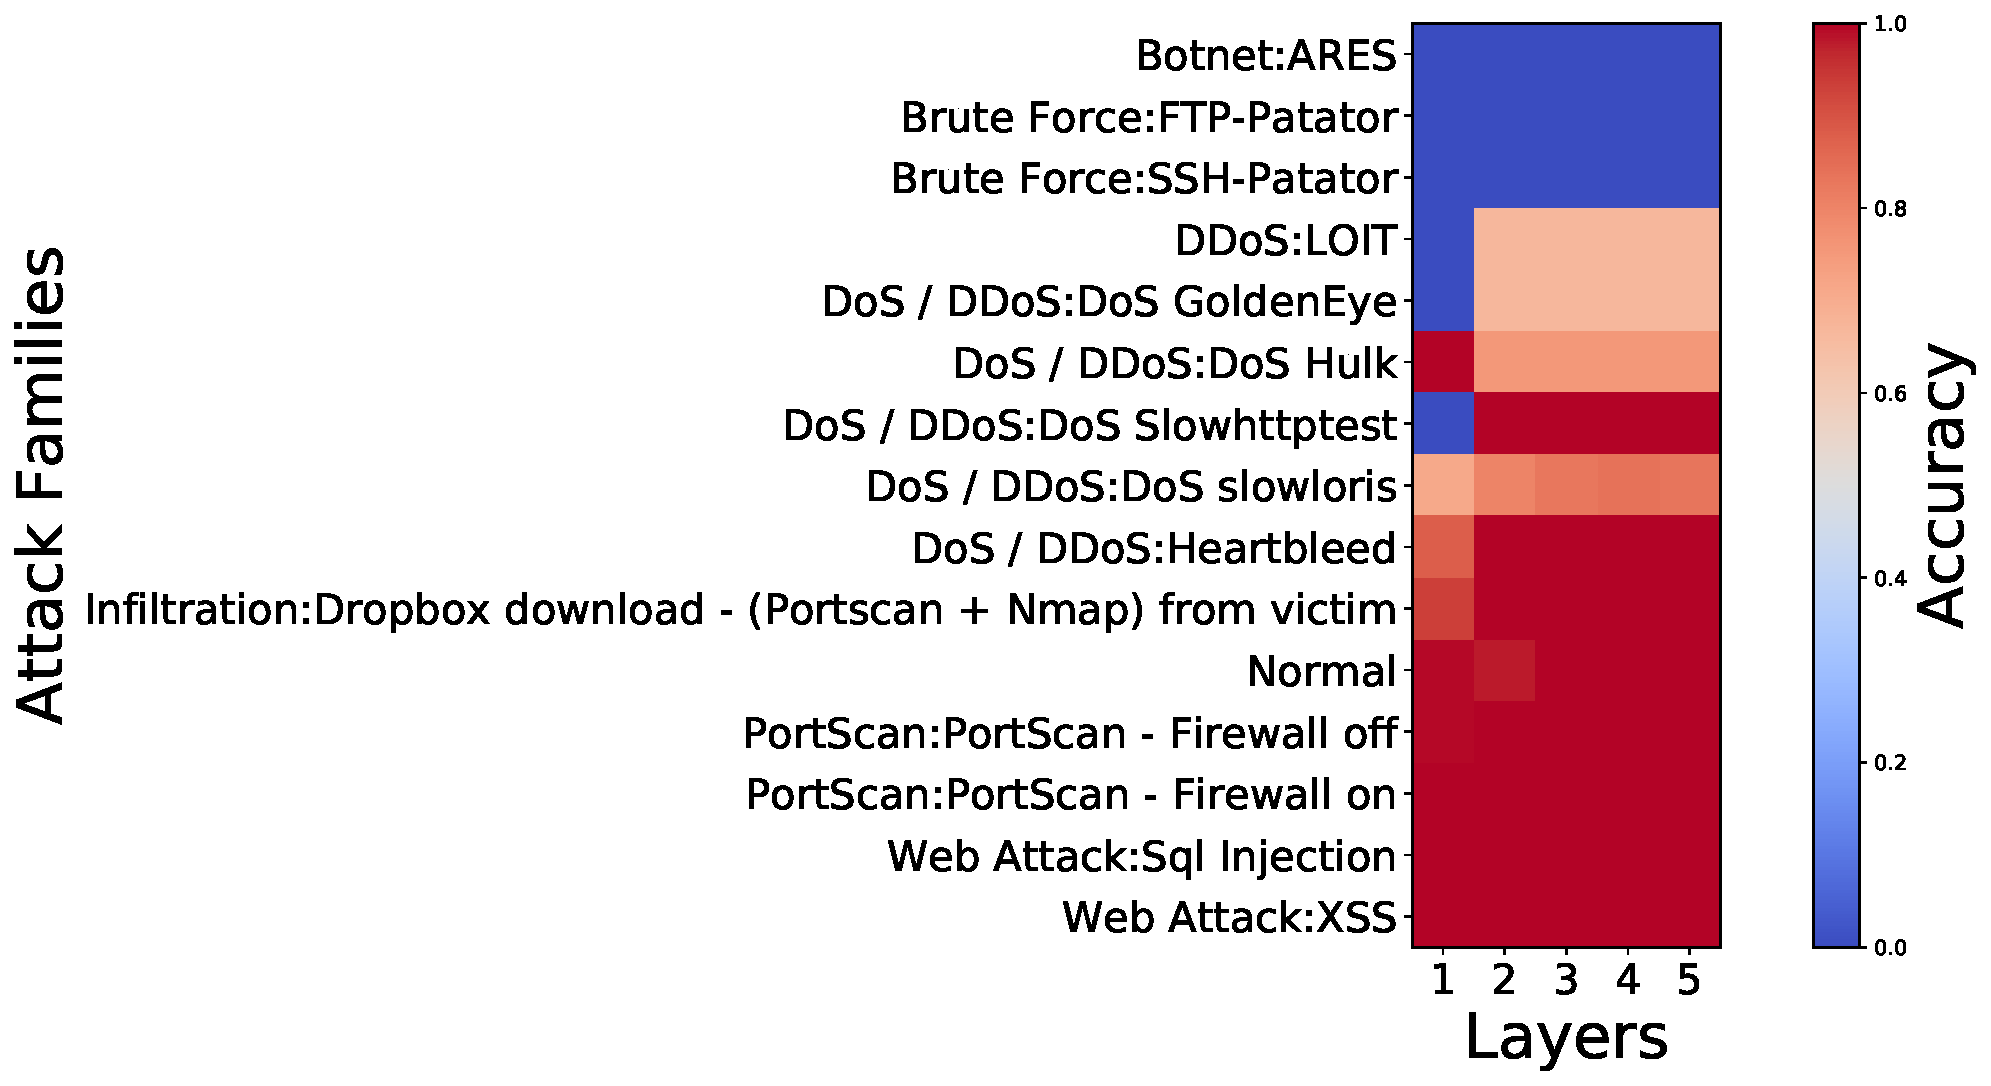
\includegraphics[width=\columnwidth]{figures/acc_multiclass_Jul10_15-18-24_gpu_0_3.pdf}
\caption{Accuracy plot multiclass.\note{red}{FM: this will change}}
\label{fig:pdp_ttl}
\end{figure}


\section{Conclusion}


\section*{Acknowledgements}
The Titan Xp used for this research was donated by the NVIDIA Corporation.

\bibliographystyle{IEEEtran}
\bibliography{biblio}

\end{document}
